\documentclass{article}

% Language setting
% Replace `english' with e.g. `spanish' to change the document language
\usepackage[english]{babel}

% Set page size and margins
% Replace `letterpaper' with`a4paper' for UK/EU standard size
\usepackage[letterpaper,top=2cm,bottom=2cm,left=3cm,right=3cm,marginparwidth=1.75cm]{geometry}

% Useful packages
\usepackage{amsmath}
\usepackage{graphicx}
\usepackage[colorlinks=true, allcolors=blue]{hyperref}

\title{AlgoWorld Token White Paper}
\author{AlgoWorld team}

\begin{document}
\maketitle

\begin{figure}[htp]
    \centering
    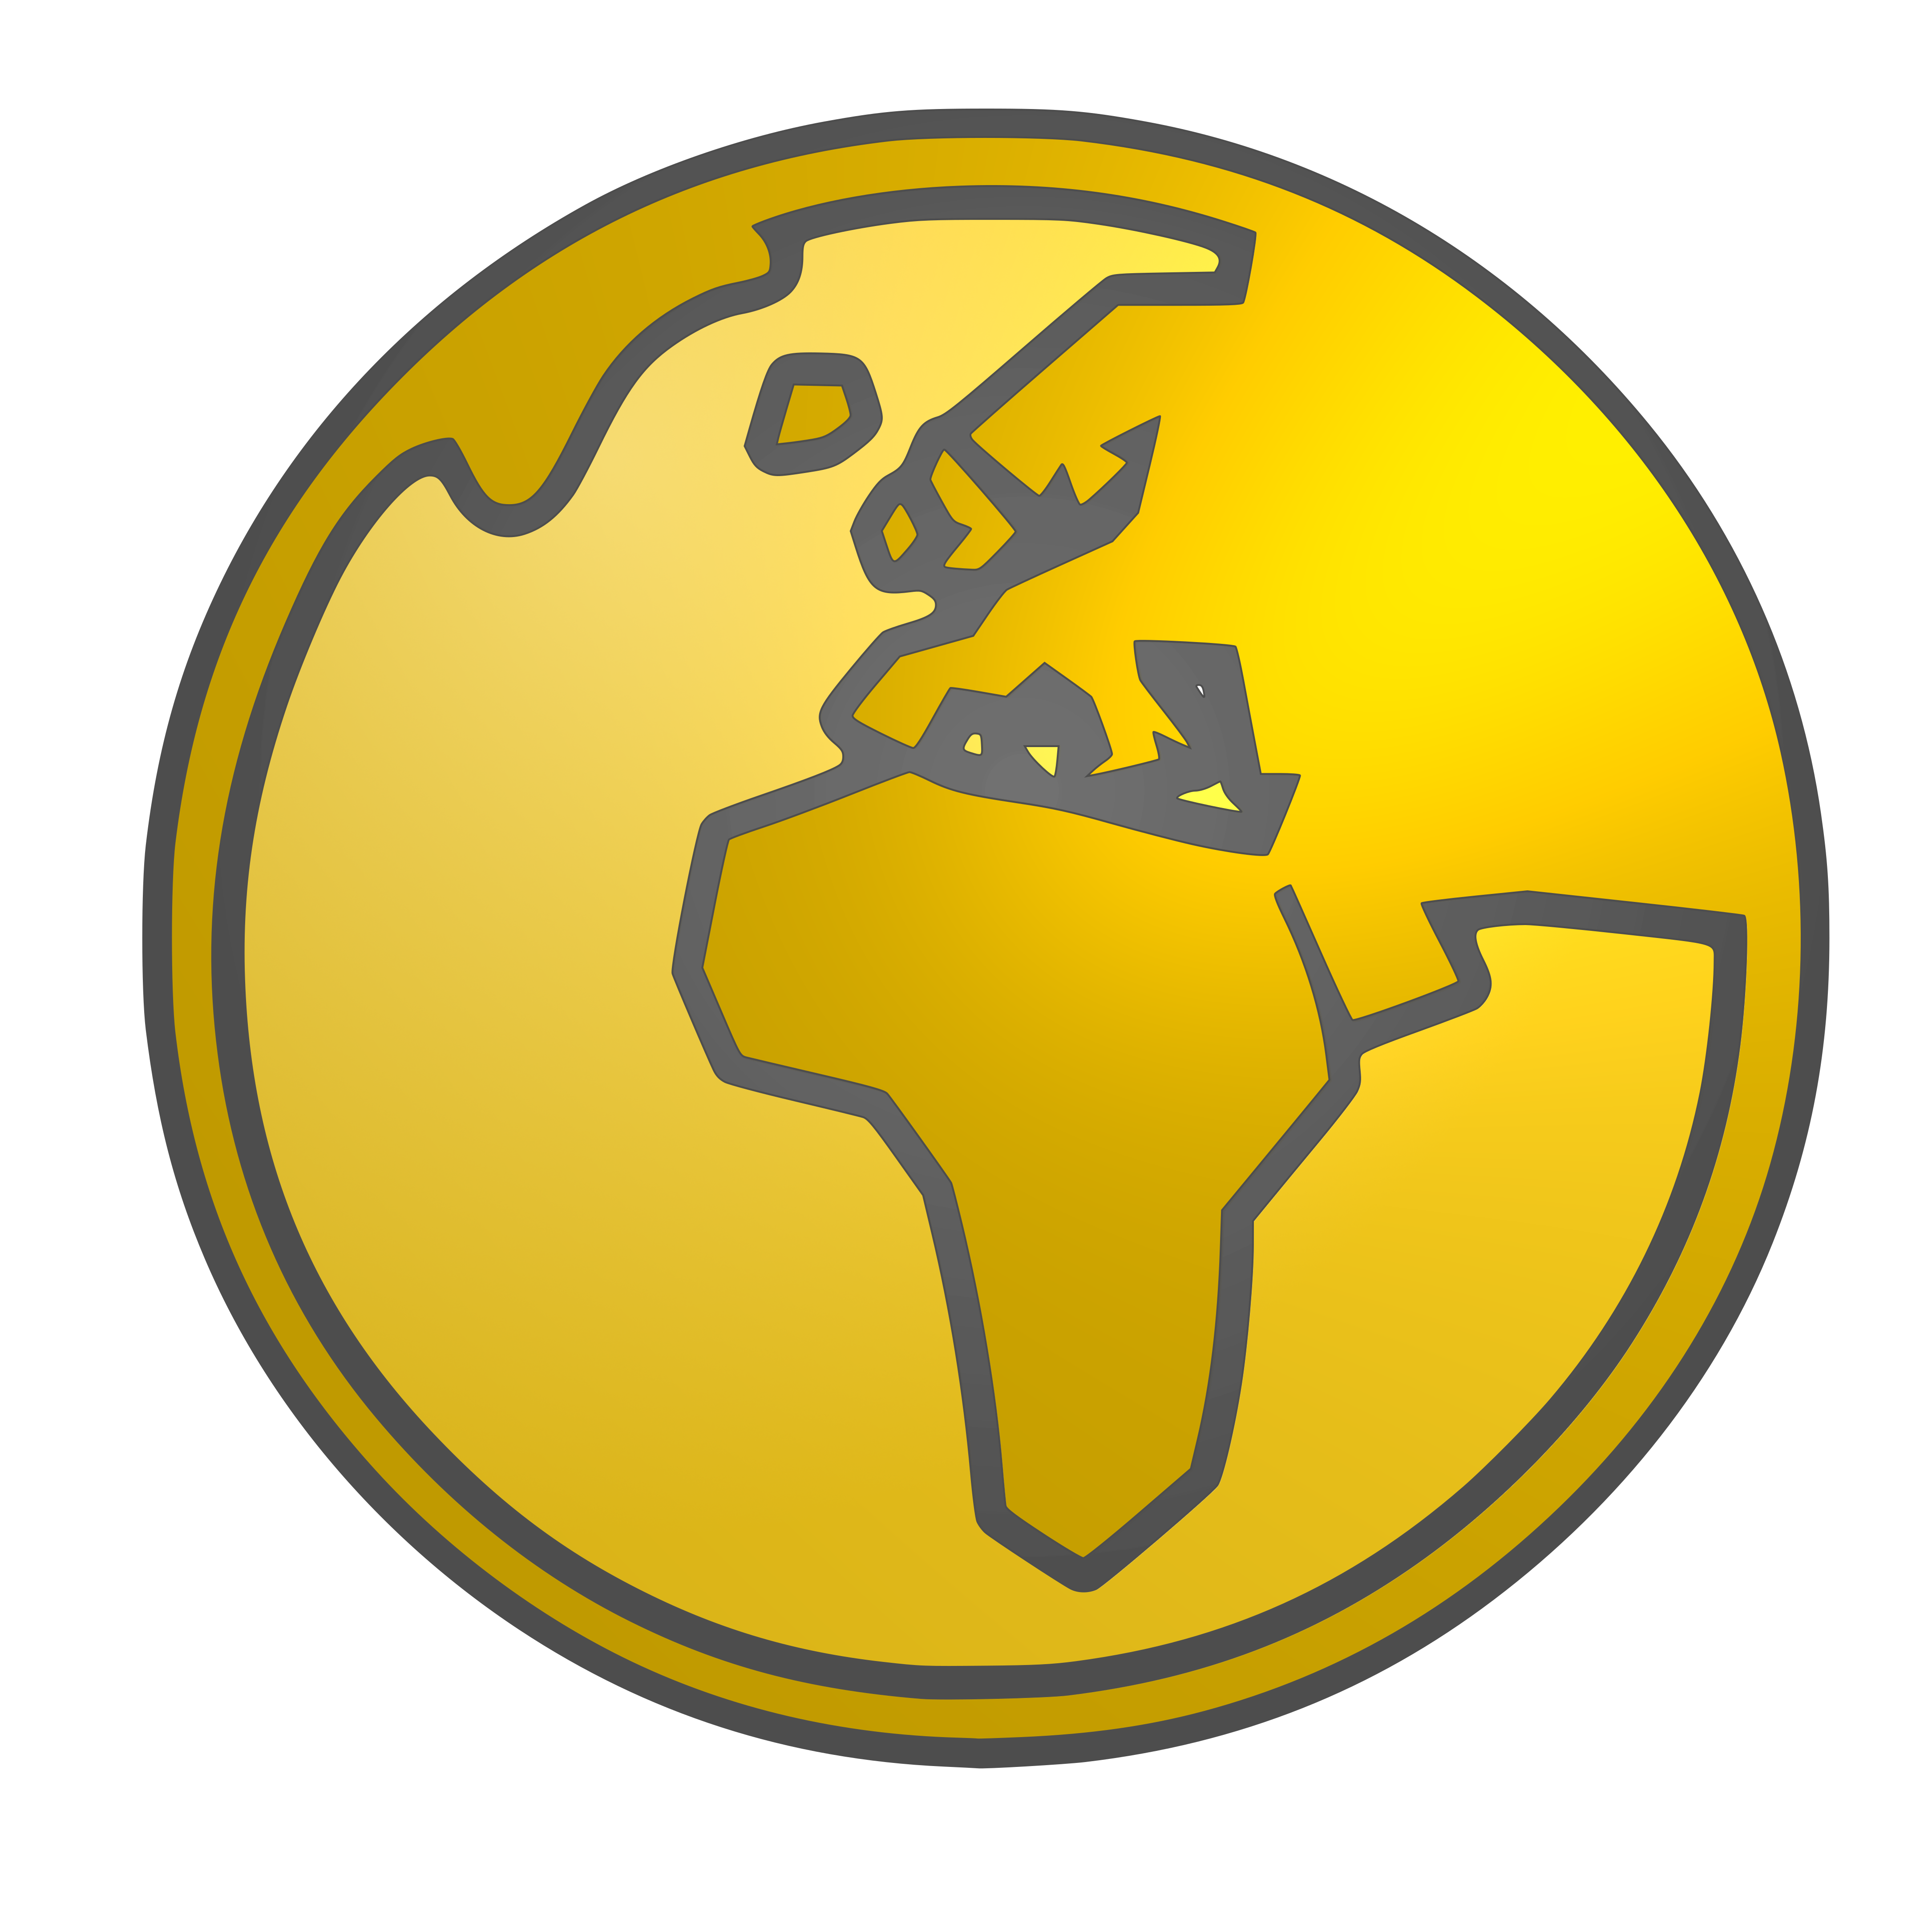
\includegraphics[width=4cm]{awt_logo.png}
\end{figure}

\begin{abstract}
The AlgoWorld Token is the utility token of the AlgoWorld NFT project, built on the Algorand blockchain. This White Paper describes the updated mechanics and distribution roadmap of this token. 

\end{abstract}

\section{Introduction}

AlgoWorld is an NFT project created in April 2021 on the Algorand blockchain. It first started with a set of 1500 NFT cards depicting the 193 United Nations countries around the world. Six special cards depicting continents and the world were added to reward the best AlgoWorld cards owners.
\\
\\
Then, a brand new feature was introduced in June 2021: the possibility to build AlgoWorld Cities (100 units cards for each city) by using the AlgoWorld Token, distributed as a reward to AlgoWorld cards owners. An additional set of 34 non-member states country cards was created in November 2021.
\\
\\
The AlgoWorld Token is a 10,000,000 units verified Algorand Standard Asset, with no decimal. The asset ID is 233939122.
The creator address is:
\\
GRV2SXHUXIHF4C5KDMC6KUH47BTBCLWJFEXM464GUTXU3BDEHE634Y6K2U.
\\
This White Paper describes the AlgoWord Cities feature and the AlgoWorld Token distribution model. 
\\
\\
Visit \href{https://www.algoworld.io}{the AlgoWorld website} to learn more about the project.

\newpage
\section{AlgoWorld Cities feature}
This feature allows members to create and upgrade new AlgoWorld Cities by using AlgoWorld Tokens. \textbf{All AWT used to build or upgrade cities are permanently removed from circulation.} 
\subsection{Building Cities}
Everyone can build new AlgoWorld Cities using AlgoWorld Tokens. Each city is a 100-units card, represented by an Algorand Standard Asset. The builder gets to choose the free of rights picture that is used for the card. 
The amount of units sent is variable, depending on the ownership of a country card of the city by the builder.
\begin{table}[ht]
\centering
\begin{tabular}{l|c}
Condition & Units sent to builder \\\hline
No country card & 50 \\
Regular country card & 55 \\
Diamond country card & 60
\end{tabular}
\caption{\label{tab:widgets}Number of city cards sent}
\end{table}
\\
\\
The units left are kept for random city packs available for sale on the AlgoWorld Explorer.
\\
\\
\textit{For instance, Joe books Boston, USA. He does not have any USA country cards. He will receive 50 Boston cards. The 50 other cards will be kept for city packs. Donald books Mexico City, Mexico. He has a Mexico diamond country card. He will receive 60 Mexico City cards. 40 cards will be kept for city packs.}
\\
\\
\textbf{Important: the same city can be built only once.}
\\
\\
The price to build a city is adjusted every month according to the number of bookings. 

\begin{itemize}
\item The price is unchanged if there are between 10 and 20 cities booked in the previous month.
\item If less than 10 cities are booked in the previous month : price decreases by 500 AWT
\item If more than 20 cities are booked in the previous month : prince increases by 500 AWT
\end{itemize}
\\\\Floor price is 1500 AWT per city.
\\\\The booking form, list of booked cities, and current city building price are available on \href{https://www.algoworld.io/city-booking}{the AlgoWorld website}.


\subsection{Upgrading Cities}
Each city can be upgraded using AlgoWorld Token on the AlgoWorld Explorer.
Sending AWT increases the influence points of a city and makes it earn more rewards (see \ref{CR} "City Rewards").
1 AWT sent adds 1 influence point to the city. 
There are 7 different ranks. The city with the highest influence is the AlgoWorld Capital. 

\begin{table}[ht]
\centering
\begin{tabular}{l|r}
AlgoWorld City rank & Influence points \\\hline
AlgoWorld Regular City & 0-99 \\
AlgoWorld Bronze City & 100-499 \\
AlgoWorld Silver City & 500-999 \\
AlgoWorld Gold City & 1000-1999 \\
AlgoWorld Platinum City & 2000-2999 \\
AlgoWorld Diamond City & 3000+ \\
AlgoWorld Capital & Highest score \\
\end{tabular}
\caption{\label{tab:widgets}City ranks}
\end{table}

\newpage
\section{AlgoWorld Token distribution}
\subsection{Allocation of AlgoWorld Token}
The 10,000,000 Tokens are allocated as follows:
\begin{table}[ht]
\centering
\begin{tabular}{l|r}
Category & Amount \\\hline
Country cards rewards & 3,000,000 AWT \\
City cards rewards & 3,000,000 AWT\\
Project fund & 1,200,000 AWT\\
Liquidity providers rewards & 1,000,000 AWT\\
Games & 550,000 AWT\\
Giveaways & 50,000 AWT\\
Early buyers compensation program & 41,500 AWT\\
Further allocation & 1,158,500 AWT
\end{tabular}
\caption{\label{tab:widgets}AWT allocation}
\end{table}

\begin{itemize}
\item Project fund is detained by the AlgoWorld team and can be sold over time. The sales will never exceed 40,000 AWT/month. This fund is also used to provide liquidity in AMM.
\item A budget of 1,000,000 AWT is introduced to incentivize AWT liquidity providers. 
\item The early buyers compensation program of 41,500 AWT aimed to give a bonus for early AWT buyers. It was fulfilled in 2021. 
\item A budget of 1,158,500 AWT (around 10\% of total supply) is not allocated yet. Its allocation will be decided later on, after consultation of the community.
\end{itemize}

\newpage
\subsection{Detailed allocation}
\subsubsection{Country rewards}
Rewards are sent weekly for each country card of the AlgoWorld collection.
The rewards distribution rate is accelerated compared to the initial roadmap, to ensure full distribution in a reasonable timeframe. Country cards rewards will be fully distributed in around 80 weeks.
\begin{table}[ht]
\centering
\begin{tabular}{l|r}
AlgoWorld Country & Rewards \\\hline
Regular country & 10 AWT/card \\
Diamond country & 100 AWT/card \\
Special card & 100 AWT/card \\
Continent card & 250 AWT/card \\
World card & 500 AWT/card \\
\end{tabular}
\caption{\label{tab:widgets}Country rewards}
\end{table}

\subsubsection{City rewards}
\label{CR}
The rewards for each city card depend on the city rank. It is reminded that each city has 100 cards. The total amount of city rewards (3,000,000 AWT) is split into three tranches of 1,000,000 AWT each.
\begin{table}[ht]
\centering
\begin{tabular}{l|r}
AlgoWorld City & Rewards \\\hline
AlgoWorld Regular City & 1 AWT/card \\
AlgoWorld Bronze City & 2 AWT/card \\
AlgoWorld Silver City & 3 AWT/card \\
AlgoWorld Gold City & 4 AWT/card \\
AlgoWorld Platinum City & 5 AWT/card \\
AlgoWorld Diamond City & 6 AWT/card \\
AlgoWorld Capital & 10 AWT/card \\
\end{tabular}
\caption{\label{tab:widgets}City rewards}
\end{table}

\begin{itemize}
\item First tranche distribution rate: weekly
\item Second tranche distribution rate: bi-monthly
\item Last tranche distribution rate: monthly
\end{itemize}

\textit{For instance, the holder of 20 cards of a Regular City will earn 20 AWT/weekly during the first tranche distribution.}

\subsubsection{Liquidity providing rewards}

AWT rewards will be sent weekly to liquidity providers. The total amount dedicated to this category is 1,000,000 AWT.
2\% of AWT provided to Tinyman Algo/AWT liquidity pool will be sent every week to each liquidity provider. This distribution rate could be changed to distribute the liquidity rewards over 2 to 4 years.

\subsubsection{Games}
Games such as treasure hunts will be organized to have roughly 100,000 AWT distributed each year.


\end{document}